
\chapter{Mes réalisations}

\section{Présentation du framework Play!}

Play! est un jeune framework qui permet de créer facilement des
applications web avec Java et Scala.
Mon stage a deux buts majeurs pour l'entreprise :

\begin{enumerate}
\item Rendre accessible à tous l'utilisation de l'outil d'infra en proposant
  une interface web ergonomique.
\item Explorer le potentiel du framework Play! pour qu'il remplace
  éventuellement du code php existant dans différents logiciels de
  l'entreprise.
\end{enumerate}

Durant mes deux premières semaines de stage, j'ai préparé des slides pour une
présentation du framework. Cette présentation met en avant les caractéristiques
de Play!, ses points forts et faiblesses, et comment il se place face aux
alternatives existantes.
L'équipe croit au potentiel du framework mais attend le résultat de
l'interface web de l'outil d'infra pour décider de remplacer le code php
existant.

\underline{\textit{Bilan}} : Cette présentation m'a permis de travailler
l'aisance orale devant un public de techniciens. J'ai pu confronter mes arguments
en faveur (ou défaveur) du framework Play! avec ceux d'autres programmeurs
expérimentés qui ont déjà utilisé plusieurs frameworks Web.

\noindent\hrulefill

La semaine suivante consiste à tester l'outil d'infra en ligne de
commande et à réfléchir à l'interface utilisateur pour l'application web (url
disponibles, dispositions des boutons et des champs de saisies).

Une nouvelle branche est ajoutée dans Mercurial pour accueillir l'application web.
Le développement peut commencer!


\section{Le déploiement}

Le déploiement doit être fonctionnel avant de développer l'application.

En effet, il se peut que les contraintes d'infrastructure empêchent
le déploiement d'une application : l'espace disque dur qui peut être insuffisant
pour accueillir l'application, l'impossibilité d'ouvrir des ports http.
Si on ne sait pas mettre à disposition une application à ses
utilisateurs (i.e. la déployer) le travail réalisé est inutile, elle n'apporte
aucune valeur.
Nous devons donc vérifier que le déploiement fonctionne bien de bout en bout.

Pour cela, une application simpliste est créée.
Elle affiche juste une page web avec du contenu statique.

Il faut maintenant héberger l'application puis automatiser le déploiement en
programmant des scripts.

\subsection{Amazon héberge l'application}

Sur Amazon Web Services, une instance EC2 portant le nom 'infra-admin-web' est
créée. C'est en fait le serveur qui hébergera l'application. Le
système d'exploitation de cette instance est Ubuntu 12.04 .
C'est une instance de type \textit{t1.micro} qui est idéale pour le type
d'application web attendue.
En effet, les clients de l'application web seront les membres de la société.
Du fait du nombre limité d'utilisateurs, environ 25 développeurs,
une puissance CPU limitée suffit.

Une instance Micro (\textit{t1.micro}) fournit une petite quantité de ressources CPU
constantes et augmente dynamiquement sa capacité CPU sur de courtes durées
lorsque des cycles supplémentaires sont disponibles. Donc elle convient bien
aux applications à moindre trafic ou aux sites consommant un nombre de cycles
significatif périodiquement.

Le schéma suivant illustre l'utilisation CPU typique d'une application web
tournant sur une instance de type \textit{t1.micro} :
\begin{figure}[H]
  \begin{center}
    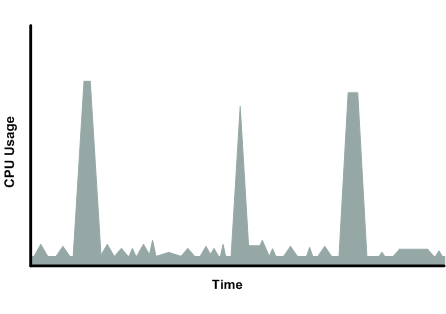
\includegraphics[scale=0.8]{cpu-usage.png} 
  \end{center}
  \caption{utilisation CPU pour une instance de type micro}
\end{figure}

Les instances de type micro sont aussi les moins chères de tous les types
d'instances proposés par Amazon. Leurs prix est de seulement 2 centimes de
dollars par heure.

\underline{\textit{Bilan}} : Découverte et première utilisation d'AWS. Ce
service de Cloud Computing fourni par Amazon est l'investissement le plus
rentable pour les jeunes entreprises. De plus en plus d'entreprises l'utilisent
car il est économique, fiable et évolutif. Avoir les droits d'accès pour piloter
AWS est une opportunité pour moi d'apprendre à maîtriser cet outil.

\subsection{Scripts Bash}

Maintenant que nous disposons d'une instance EC2 réservée pour l'application
web, il faut automatiser les actions récurrentes qui devront être effectuées.

Quatre scripts Bash sont créés pour exécuter les tâches récurrentes :
deploy.sh, start.sh, stop.sh et restart.sh pour respectivement déployer
l'application web, la démarrer, l'arrêter et la redémarrer.

deploy.sh est un script qui se trouve sur la machine local.
Ce script package l'application puis la copie sur l'instance EC2 via scp.
Les scripts start.sh, stop.sh et restart.sh se trouvent sur l'instance EC2 et
peuvent être appelés à distance via ssh.

\underline{\textit{Bilan}} : Mes connaissances en Bash et sur l'environnement
Linux m'ont permis de créer rapidement ces scripts d'automatisation de
déploiement.

\section{Premier concept de webapp : appeler l'outil d'infra comme une commande
  shell}
\noindent Les objectifs de la première version de la webapp sont les suivants :
\begin{enumerate}
\item La webapp exécutera l'outil d'infra en ligne de commande comme un
  programme externe.
\item La webapp doit permettre d'exécuter deux commandes en parallèle.
\end{enumerate}

Le code côté serveur est écrit en Scala.
Puisque toute classe Java peut être naturellement instanciée dans du code Scala,
c'est la classe Java ProcessBuilder qui est utilisée pour exécuter
l'outil d'infra comme programme externe.
Qu'en au code côté client, il doit afficher la sortie de la commande dans le
navigateur.

Une contrainte apparaît :
Certaines commandes de l'outil d'infra prennent beaucoup de temps à s'exécuter.
L'output de la commande doit donc être affichée au fur et à mesure de son
exécution. Pour ce faire :\\
\textit{Côté serveur}, un BufferedReader récupère dynamiquement la sortie de la commande.\\
\textit{Côté client}, du JavaScript affiche progressivement le résultat.

Le point restant est la communication entre le serveur et le navigateur du
client pour afficher dynamiquement du contenu dans la page web.

\subsection{Communications asynchrones pour une application web temps réel}
%\textit{\underline{Communications asynchrones pour une application web temps réel}}\\

Dans une application Web traditionnelle, lorsque l'utilisateur effectue une
action, celle-ci est exécutée et le navigateur attend le résultat pour rendre
la main à l'utilisateur. Lorsque cette action requiert un calcul coûteux
au serveur, cela occasionne des délais et une attente pour le client.

Le mode asynchrone élimine cette attente. Les requêtes au serveur sont lancées
sans que soit suspendue l'interaction avec le navigateur et la page est mise à
jour lorsque les données requises sont disponibles.

La première solution bien connue pour disposer de ce comportement asynchrone est
\textit{Ajax}.
\textit{Ajax} est une technologie permettant de créer des applications qui simulent un
comportement temps réel. Le navigateur envoi une requête HTTP à intervalle
régulier et reçoit une réponse.
Il existe aujourd'hui des alternatives à \textit{Ajax} pour voir des données se
mettre à jour dans sa page web sans appuyer sur le bouton refresh.

La webapp de l'outil d'infra utilise des \textit{WebSocket}.
C'est une autre technologie web, bien plus récente, qui permet de créer de vrais
applications temps réel.
Alors que le protocole HTTP opère par une succession de requêtes et réponses
alternatives, \textit{WebSocket} est bidirectionnel : une connexion statique s'établit
entre le serveur et le client et les deux parties envoient des données à leur
convenance.
C'est un authentique canal de communication bidirectionnel (push depuis le
serveur) transparent pour les firewalls, proxy, et routeurs.
Il n'y a aucune latence réseau lors des transmission, les performances réseaux
qu'elle offre est l'un de ses gros points forts.
Le framework Play! fournit une bibliothèque complète pour utiliser les
\textit{WebSockets}.
La webapp fait donc usage des \textit{WebSockets} pour récupérer dynamiquement le
résultat de la commande et l'afficher dans le navigateur.

Pour chaque nouvelle page ouverte, une WebSocket est créée.
Deux utilisateurs peuvent alors exécuter leur commande en parallèle sans
blocage ni intercalage des logs des commandes.

Voici une capture d'écran de l'interface web disponible avec la première version
de la webapp :
\begin{figure}[H]
  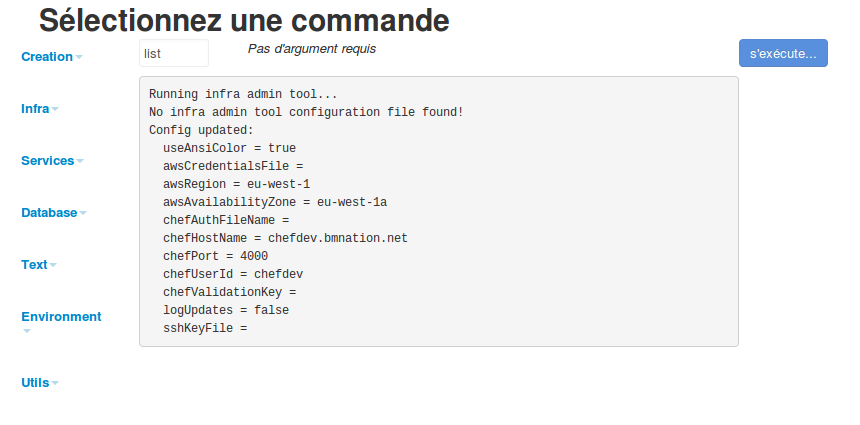
\includegraphics[width=\textwidth]{webapp-processbuilder.png}
  \caption{Exécution de la commande ``list'' avec la première version de la webapp}
\end{figure}

\underline{\textit{Bilan}} :
\begin{itemize}
\item Le développement est rapide avec Play!. Le rechargement à
  chaud de l'application et l'utilisation du langage évolué Scala permettent de
  gagner beaucoup de temps.  
\item Les interactions côté client se font en JavaScript et
  je gagne en aisance à programmer avec ce langage que je connais à peine.
\item  Découverte des WebSocket, cette technologie de dialogue client/serveur
  bidirectionnelle ouvre de belles perspectives à de nouvelles fonctionnalités
  Web.
\end{itemize}

\section{Transformer l'outil d'infra en bibliothèque}

\underline{\textit{La demande}} : Transformer l'outil d'infra en bibliothèque pour ne plus
lancer un processus séparé et donc une JVM à chaque exécution de commande.
Mais, très important, l'outil doit toujours fonctionner en ligne de
commande.

\underline{\textit{L'objectif}} : Générer un jar de l'outil d'infra pour ensuite
l'intégrer à l'application web. Les méthodes de l'outil d'infra seront
directement accessibles dans le code source de la webapp.

La transformation de l'outil d'infra en API impose plusieurs changements qui
sont présentés dans les sous-sections qui suivent.

\subsection{Des singletons transformés en simples classes}

Toutes les classes étaient des services. Elles étaient toutes des singletons.
Les services proposent des méthodes utilitaires et n'ont pas d'état. Il était
donc logique d'avoir des singletons car nous n'avions pas besoin de plus d'une
instance par service. 

De même, il existait un singleton Logger qui était utilisé par tous les autres
singletons afin de logguer leurs différentes actions.

Dans l'outil d'infra en ligne de commande, un seul logger suffisait, un simple
logger qui enregistre tout dans un fichier.
Mais pour que l'outil se transforme en API, l'utilisateur doit avoir le
contrôle sur le logger. L'utilisateur doit pouvoir choisir son logger, il doit
pouvoir en utiliser plusieurs si il souhaite.

C'était en effet le cas de l'application web qui allait être le premier
programme à utiliser l'API. L'application web a besoin de plusieurs
loggers. En fait, elle a besoin d'un logger par internaute.
Une nouvelle instance du Logger est créée pour chaque nouvel internaute afin
que les résultats des commandes lancées par un internaute soient isolés dans son
propre fichier. Les logs des internautes ne doivent pas être mélangés.

Un refactoring important a permis la transformation de l'outil d'infra en API.
Tous les singletons sont transformés en simples classes.
Puisqu'il n'existe plus de singleton, les constructeurs de ces classes prennent
alors en paramètre les instances d'autres classes dont elles dépendent.

Par chance, l'outil d'infra a été développé avec un langage statiquement
typé, Scala en l’occurrence.
Lorsqu'un singleton se transforme en simple classe, le code extérieur qui
utilisait ce singleton doit changer sa façon de l'appeler.
Grâce au typage statique, Eclipse affichait les erreurs de compilation dans
les différents fichiers faisant usage de la classe modifiée. Il suffisait alors
de suivre ces erreurs et de les corriger.

\underline{\textit{Bilan}} : Cette tâche fut assez longue à faire mais il n'y
avait pas de complexité particulière, le résultat était assuré.
En plus de l'objectif premier qui était de pouvoir utiliser l'outil d'infra en
tant qu'API, les dépendances entre les classes sont maintenant clairement
exposées ce qui facilite la compréhension du code.

\subsection{Libération mémoire du cache}

L'outil faisait aussi utilisation d'un cache pour l'optimisation de méthodes
appelées plusieurs fois durant l'exécution d'une même commande.

Puisque ce programme était conçu pour exécuter une seule commande, la
consommation mémoire de ce cache ne posait pas problème.
À la fin de l'exécution de la commande, le programme se termine et la JVM
se charge de libérer la mémoire allouée.

Dans le cadre d'une API, le problème est différent. Le client qui utilise l'API
de l'outil d'infra ne souhaite peut-être pas exécuter une seule commande.
Si le client exécute plusieurs commandes successives, le cache grossit pour
chaque nouvelle commande exécutée et consomme de plus en plus de mémoire.

C'est le cas de l'application web dont la durée d'exécution est \textit{supposée}
infinie. Une fois mise en production, l'application web doit être
continuellement disponible pour les utilisateurs. Seul le déploiement d'une
nouvelle version de l'application web doit engendrer son redémarrage.

Pour corriger ce problème, les données relatives à une commande sont supprimées
du cache lorsque l'exécution de cette commande se termine.

\underline{\textit{Bilan}} : Ce problème de cache non libéré n'a été détecté
qu'une fois l'application web mise en ligne. Après quelques jours
d'utilisation, une exception java.lang.OutOfMemoryError avait été lancée par la
JVM du serveur. Ce problème ne s'est pas reproduit une fois la solution mise en
place. L'option -XX:+HeapDumpOnOutOfMemoryError a aussi été rajouté au lancement
de la JVM pour récupérer à l'avenir une description complète de l'état du tas
(heap) de la mémoire si une même exception se produisait.

\subsection{Des types de retour plus riches}

Plusieurs méthodes de haut niveau, directement appelées par le main de l'outil
d'infra, ne renvoyaient rien car le seul retour utile était imprimé
sur stdout et stderr. Ces méthodes de haut niveau font maintenant parti de l'API
de l'outil d'infra et peuvent être appelées en dehors du main par n'importe
quelle autre méthode.
Les types de retour des méthodes de l'API ont donc été enrichis.

Par exemple, la commande 'list' affiche sur la sortie standard la liste de
toutes les infrastructures existantes.
Son type de retour était Unit (void en Java) et devient Seq[Infra] (en Java, le
type le plus proche serait List<Infra>).
Le client de l'API peut alors se servir de la liste des infrastructures retournée.

\underline{\textit{Bilan}} : L'application web utilise le jar de l'outil d'infra
pour accéder à ses méthodes. Il n'est plus nécessaire de lancer un processus
séparé pour exécuter une commande.

\section{Les pages de la nouvelle webapp}
L'application web possède trois pages :
la page \textit{Commands}, la page \textit{Infras} et la page \textit{History}.

\subsection{La page Commands}

C'est la page principale du site. C'est aussi la plus utilisée car c'est à
travers cette page qu'il est possible d'exécuter n'importe-quelle commande de
l'outil d'infra. 

\begin{figure}[H]
  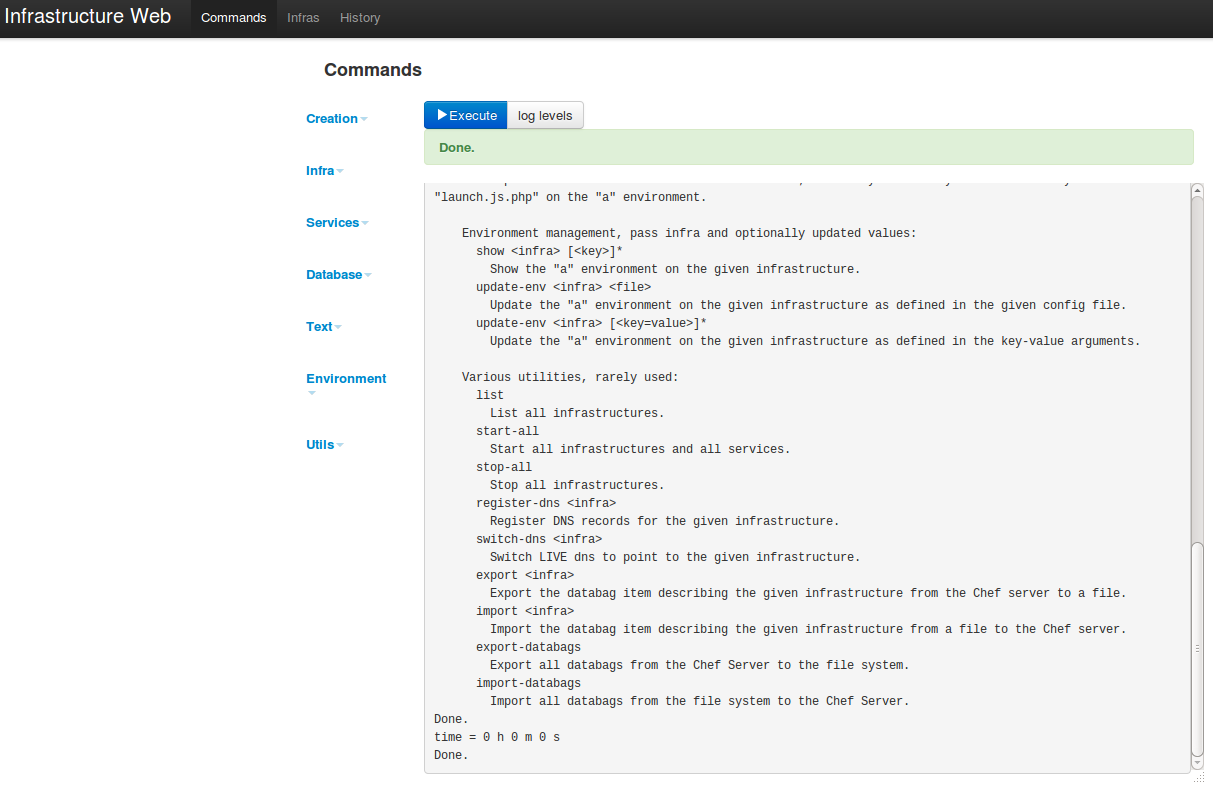
\includegraphics[width=\textwidth]{commands.png}  
\end{figure}

\subsection{La page Infras}

La page Infras est un tableau de bord des infrastructures existantes.

Les informations exposées sont sont celles de l'outil d'infra. Tous les
attributs ne sont pas exposés à l'utilisateur. Si l'utilisateur souhaite
consulter l'ensemble des attributs d'une infrastructure, il peut le faire en se
connectant sur Chef car c'est Chef qui stocke toutes les informations relatives
à une infrastructure.

Le chargement des attributs pour l'ensemble des infrastructures existantes met
environ 5 secondes à s'exécuter sur l'instance EC2 qui héberge la webapp.
Un icône animé de chargement indique à l'utilisateur de patienter.

\begin{figure}[H]
  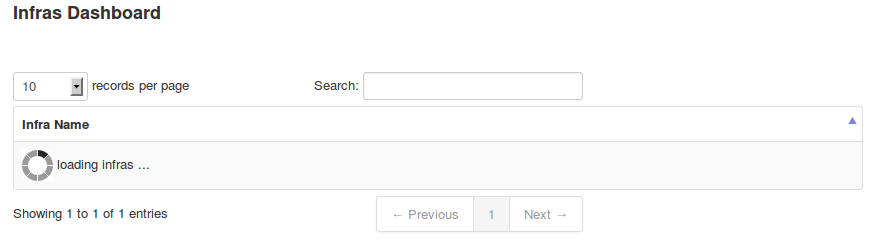
\includegraphics[width=\textwidth]{infras-dashboard-loading.png}  
  \caption{Chargement des infrastructures}
\end{figure}

Une fois les informations des infrastructures chargées, tous les noms d'infra
sont affichés sous forme de tableau.
\begin{figure}[H]
  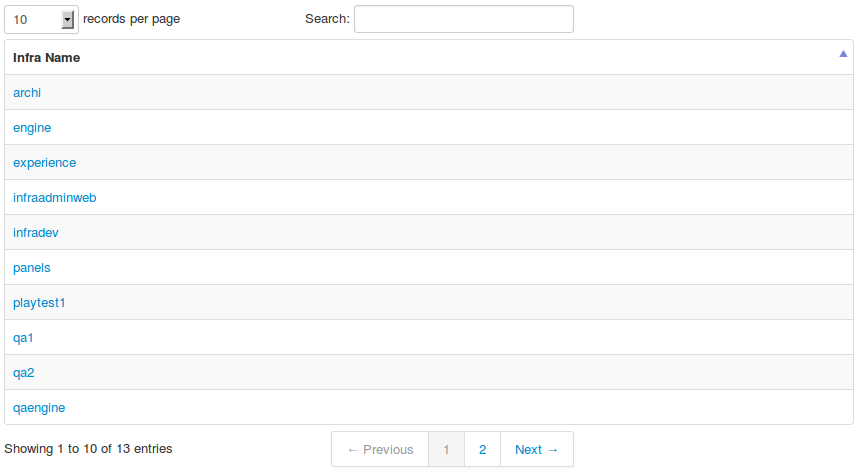
\includegraphics[width=\textwidth]{infras-dashboard.png}  
  \caption{les noms d'infrastructure présentés dans un tableau}
\end{figure}

L'utilisateur peut cliquer sur l'infrastructure qui l'intéresse.
Un deuxième tableau se présente à l'utilisateur dans lequel il peut consulter
les versions des différents services de l'infrastructure sélectionnée.
\begin{figure}[H]
  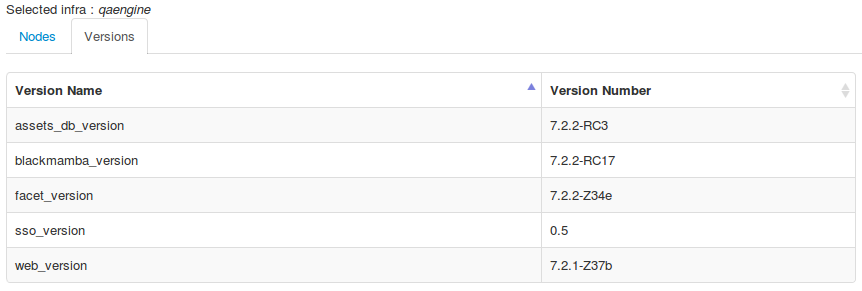
\includegraphics[width=\textwidth]{infra-versions.png}  
  \caption{les versions des services de l'infrastructure qaengine}
\end{figure}

Les nœuds appartenant à l'infra sélectionnée sont aussi accessibles via un
onglet \textit{Nodes}. 
Ce tableau nous affiche des informations intéressantes pour chaque nœud telles
que l'ID de l'AMI (Amazon Machine Image), le type d'instance EC2 qui héberge le
nœud, le hostname que l'on peut utiliser si on souhaite se connecter en ssh sur
l'instance du nœud, et enfin la liste des Security Groups.

\begin{figure}[H]
  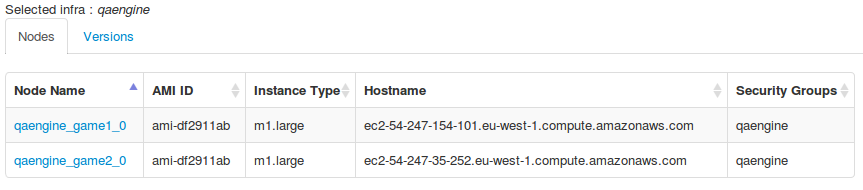
\includegraphics[width=\textwidth]{infra-nodes.png}  
  \caption{les nœuds de l'infrastructure qaengine}
\end{figure}

L'utilisateur peut cliquer sur le nœud qui l'intéresse.
Un troisième et dernier tableau se présente à l'utilisateur dans lequel il peut
consulter les rôles Chef appliqués au nœud sélectionné.

\begin{figure}[H]
  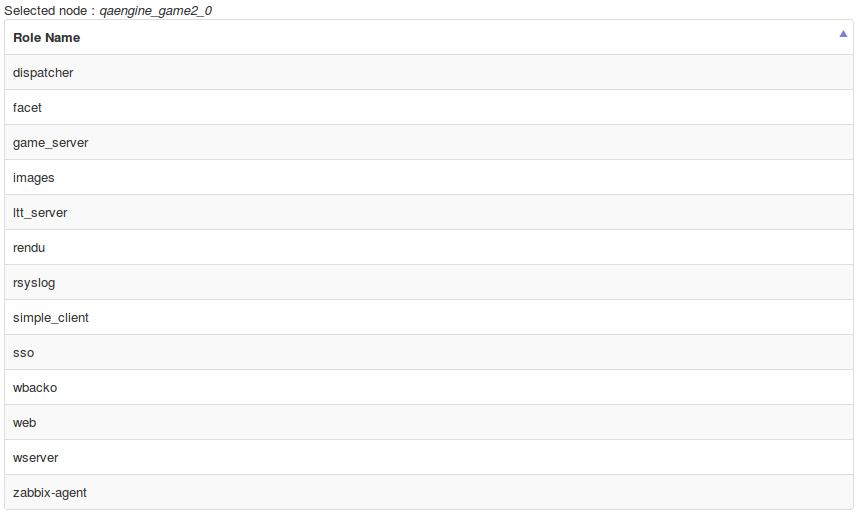
\includegraphics[width=\textwidth]{node-roles.png}  
  \caption{Les rôles du nœud qaengine\_game2\_0}
\end{figure}

\subsection{La page History}

La page History affiche l'historique des commandes exécutées.
Les 100 dernières commandes sont présentées dans un tableau dans l'ordre
chronologique inverse de leur date d'exécution, en commençant par l'exécution de
la commande la plus récente.
Ces 100 commandes ne sont pas persistées en base de données. Elles sont stockées
dans une file. Lorsqu'une 101 ème commande est ajoutée à la file, la première
est supprimée afin de ne conserver que les 100 dernières commandes. Cet élément
supprimé de la file sera récupéré par le garbage collector.
À l'avenir, il est prévu de rajouter la notion d'utilisateur avec un système
d'authentification, afin d'avoir un audit complet.

Cette page affiche deux informations supplémentaires qui sont le nombre de
pages \textit{commands} actuellement ouvertes (lorsqu'on déploie une nouvelle
version, on prévient par mail le nouveau déploiement et on vérifie que le nombre
de pages \textit{commands} ouvertes vaut 0) et le nombre de commandes
actuellement en cours d'exécution.

\begin{figure}[H]
  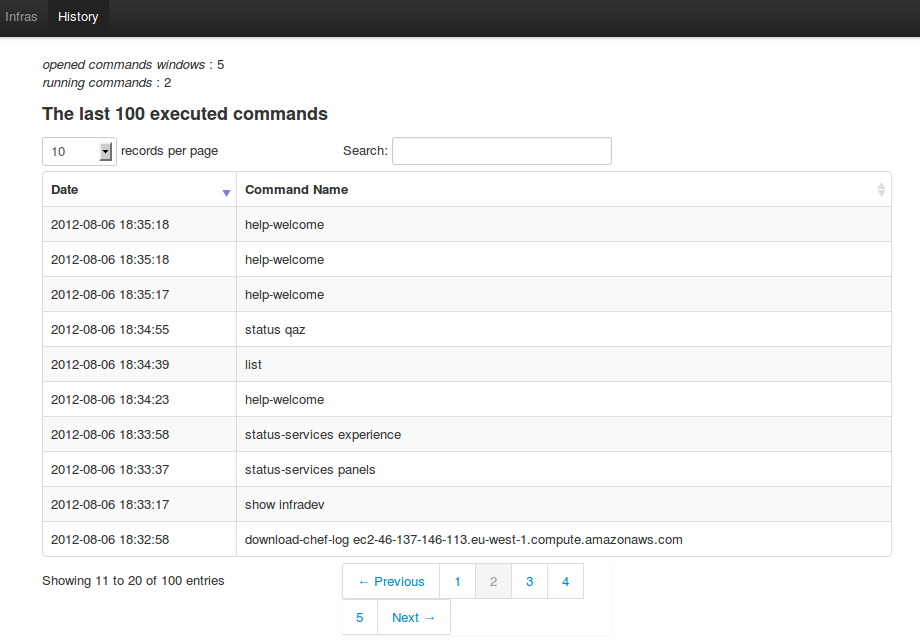
\includegraphics[width=\textwidth]{history.png}  
  \caption{Historique des 100 dernières commandes exécutées}
\end{figure}

\section{Composants de la page commands}

La webapp propose 30 commandes réparties dans 7 catégories différentes.
Voici un tableau récapitulatif de ces commandes.\\\\
\begin{tabular}{|c|c|c|c|c|c|c|c|c|c|c|c|}
  \hline
  \begin{bf}Catégories\end{bf} & \multicolumn{5}{c|}{\begin{bf}Commands\end{bf}} \\
    \hline
    Creation & create & migrate \\
    \cline{1-5}
    Infra & start & stop & status & destroy \\
    \cline{1-5}
    Services & start-services & stop-services & restart-services & status-services \\
    \cline{1-5}
    \multirow{2}*{Database} & deploy-db & liquibase-install & liquibase-sync\\
    \cline{2-4}
    & liquibase-update & run-migration-tool  \\
    \cline{1-3}
    Text & management & deploy-wti \\
    \cline{1-4}
    Environment & show & update-env-file & update-env \\
    \cline{1-6}
    \multirow{3}*{Utils} & help & free & list & start-all & stop-all \\
    \cline{2-6}
    & register-dns & switch-dns & export & import & export-databags\\
    \cline{2-6}
    & import-databags \\
    \cline{1-2}
\end{tabular}


\subsection{Champs de saisie}

%% \begin{figure}[H]
%%   \begin{center}
%%     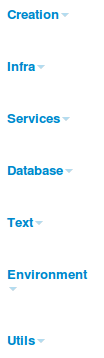
\includegraphics[scale=0.5]{categories.png} 
%%   \end{center}
%%   \caption{Les 7 catégories de commandes qui sont des listes déroulantes} 
%% \end{figure}

Lorsque l'utilisateur clique sur l'une des commandes d'une catégorie, il voit
apparaître en haut de l'application plusieurs champs de saisie qui décrivent les
arguments que doit recevoir la commande.
Il y a un champ de saisie pour chaque argument.
La commande \textit{restart-services} prend le nom d'une infra en
arguments. Elle possède donc un champ ``infra...''.
La commande \textit{update-env-file} prend le nom d'une infra et le chemin du
fichier de description de mise à jour de l'infra en arguments. Elle possède donc
un champ ``infra...'' et un sélecteur de fichier.

\begin{figure}[H]
  \begin{center}
    
\includegraphics[scale=0.5]{champ-update-env-file.png} 
  \end{center}
  \caption{Commande update-env-file} 
\end{figure}

\underline{\textit{Bilan}} : Ce nombre conséquent de commandes implique d'avoir
une grosse quantité de code HTML pour disposer tous les champs sur la
page web. Play! propose un système de templating qui permet de créer des
fonctions qui génèrent du code HTML depuis le serveur et permet d'éviter la
duplication de code. Le code ainsi créé est plus compact, plus facile à
comprendre et à maintenir.

\subsection{Sélecteur de fichier}

Un sélecteur de fichier est ajouté pour les commandes \textit{create},
\textit{migrate} et \textit{update-env-file} de l'outil d'infra.

Lorsque l'utilisateur clique sur le bouton 'Execute', le fichier sélectionné est
uploadé vers le serveur et la commande elle-même est exécutée côté serveur 
en utilisant le fichier qui vient d'être téléchargé.
Du code Ajax est utilisé pour ne pas avoir besoin de recharger la page lors de
l'envoie du fichier.
Ainsi le client peut recevoir l'output de la commande dans la page web.

\underline{\textit{Bilan}} : L'utilisation des \textit{WebSocket} est inadaptée
pour uploader un fichier. \textit{Ajax} convient parfaitement pour ce type de
tâche. Il fallait tout de même faire attention à ce que la commande ne soit
exécutée qu'une fois le fichier complètement téléchargé.

\section{Restructuration du code JavaScript}

La quantité de code JavaScript est devenue conséquente. Une restructuration du
code s'impose pour améliorer sa lisibilité, simplifier sa maintenance et
faciliter l'ajout de nouvelles fonctionnalités.

%% liens pour remplir les sous section RequireJS et CoffeeScript 
%% http://www.techno-science.net/?onglet=glossaire&definition=5410
%% http://pullrequest.org/2012/01/04/requirejs.html
%% http://yannesposito.com/Scratch/fr/blog/2011-01-03-Why-I-sadly-won-t-use-coffeescript/


\subsection{RequireJS}

Dans un langage de programmation comme Java, on ne se soucie pas du chargement
des dépendances. Il suffit de les définir (import java.utils.Collection par
exemple) et la JVM s'occupe de charger les modules de façon complètement
transparente pour le développeur.

Au contraire de ces langages évolués, la gestion des dépendances n'est pas
une tâche simple en JavaScript.
JavaScript ne possède pas de système de modules intelligent, ce qui rend le
découpage de code difficile.

Prenons un exemple. Les dépendances sont représentées comme des flèches du
module du client à gauche jusqu'au module requis à droite :

module1 $\rightarrow$ module2 $\rightarrow$ module3, module4 

En JavaScript, à chaque fois que module1 est utilisé, tous les autres modules
doivent être importés dans le bon ordre de la façon suivante :
%% mettre balise de code JavaScript à la place
\lstset{language=XML}
\begin{lstlisting}
  <script type="text/javascript" src="module4"></script
  <script type="text/javascript" src="module3"></script>
  <script type="text/javascript" src="module2"></script>
  <script type="text/javascript" src="module1"></script>
\end{lstlisting}

Heureusement, il existe quand même des moyens de définir de telles hiérarchies de
dépendances en JavaScript. RequireJS est une bibliothèque qui rend possible la
définition de dépendances entre modules de manière appropriée pour le navigateur.
RequireJS est une sorte de \#include/import/require pour JavaScript.\\
Voici un extrait de code de l'application utilisant RequireJS :
\lstset{language=JavaScript}
\begin{lstlisting}[caption=Définition du module commands avec RequireJS]
  define(
  // La liste des dépendances 
  // en python: import jquery, bootstrap-typeahead, bootstrap-button, bootstrap-dropdown
  ['jquery', 'bootstrap-typeahead', 'bootstrap-button', 'bootstrap-dropdown'], 
  function(dollar) { 
    // RequireJS assure que les quatre dépendances seront chargées et accessibles à
    // l'intérieur de la fonction.
    
    // définition de la fonction commands
    function commands(webSocketURL, listInfrasSocketURL) = {
      ...
    }
    
    // Utilisation du return pour exporter la fonction commands.
    // Tout ce qui n'est pas exporté reste privé au module.
    return commands;
  }
\end{lstlisting}


%% // in python: import myModule1, myModule2
%% requirejs(['myModule1', 'myModule2'], function (m1, m2) {


\subsubsection{Bénéfique pour la qualité du code}

\textit{\underline{Des APIs et namespace plus propres}}\\

La définition de modules avec RequireJS force le développeur à réfléchir à la
façon dont le module va partager les variables. Forcer le développeur à décider
ce qu'il veut exposer et quels sont les détails d'implémentation spécifiques
qui doivent être cachés conduisent à une meilleure encapsulation du code.

En plus, lorsque le développeur importe un module avec RequireJS, les propriétés
et méthodes exportées par le module sont accessibles à travers une variable
``package''. Ça permet à deux modules différents d'exporter un attribut avec le
même nom sans que l'un d'eux ne cache la valeur de l'autre.

%% http://imediava.wordpress.com/
%% http://imediava.wordpress.com/2012/04/23/intro-require-js/

\subsubsection{Bénéfique pour les performances}

\textit{\underline{Charger de plus petites ressources avec moins de requêtes}}\\

Deux principaux facteurs affectent le chargement d'une page :
\begin{itemize}
\item La taille des ressources. Le temps de chargement augmente avec la taille
  des ressources.
\item Le nombre de ressources. Plus il y a de ressources plus le nombre de
  requêtes augmente.
\end{itemize}

La meilleur approche pour gérer le premier cas est de ``minifier'' le code.
Minifier consiste à supprimer tous les caractères du code qui sont seulement
utiles pour rendre le code plus lisible (des espaces et retours à la ligne
entre autres).

Pour diminuer le nombre de requêtes HTTP, la solution habituelle (sans rentrer
dans la mise en cache) est de regrouper tous les fichiers dans un seul sans
modifier le code. De cette manière, le nombre de requêtes requises pour
récupérer les ressources du serveur est réduit à une seule.

RequireJS fournit un outil pour automatiquement minifier et
regrouper tous les modules en un seul. Cet outil est capable de minifier chaque
fichier CSS du projet et minifier et regrouper tous les fichiers JavaScript dont
les dépendances ont été définies en tant que module RequireJS.

\underline{\textit{Bilan}} : L'utilisation de \textit{RequireJS} était devenu
indispensable sans quoi la gestion des dépendances serait devenue un vrai
labyrinthe. Il est tout de même dommage de ne pas disposer de système de package
en JavaScript et de devoir faire recours à des bibliothèques tierces.

%% Peut-être ne pas mettre de section CoffeeScript ça fera trop de technologies
%% auxquelles je parle
\subsection{CoffeeScript}

Pour éviter de retomber dans les nombreux pièges rencontrés au cours du
développement de la partie cliente en JavaScript, j'ai décidé d'utiliser
CoffeeScript à la place de JavaScript.

CoffeeScript est un langage influencé par ruby qui fournit, entre autres choses,
les compréhensions de listes, une meilleure gestion des variables sans polluer
le namespace et plein d'autres outils qui rendent le développement JavaScript
plus simple. CoffeeScript compile vers du JavaScript lisible et bien formaté,
ce qui facilite le débugage.
Tout le code JavaScript écrit jusqu'ici est traduit en CoffeeScript.
Le code est plus concis (gain de $\sim$15\% pour le nombre de lignes de code) et le
développement plus fluide.

\underline{\textit{Bilan}} : CoffeeScript rend l'écriture de Javascript plus
plaisante et plus concise.

\section{Messages Done et Failed}

Lorsqu'une commande se termine, l'utilisateur reçoit un message \textbf{Done} si la
commande a réussi ou un message \textbf{Failed!} si la commande a échoué.

\begin{figure}[H]
  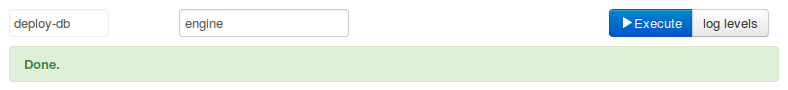
\includegraphics[width=\textwidth]{cmdDone.png}
  \caption{Déploiement réussi de la base de données pour l'infra engine}
\end{figure}

Un message \textbf{Failed!} est accompagné de l'exception Scala émise par
l'application.

\begin{figure}[H]
  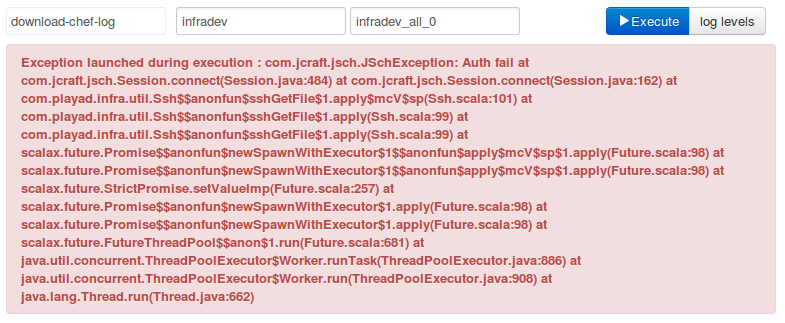
\includegraphics[width=\textwidth]{cmdFailed.png}
  \caption{Échec de la récupération des logs Chef sur le nœud infradev\_all\_0.\\
    L'application ne peut apparemment pas se connecter sur l'instance EC2 de
    ce nœud car l'authentification a échoué}
\end{figure}

\underline{\textit{Bilan}} : Ce message est mis en avant en haut de page,
l'utilisateur ne peut pas le manquer.
Il n'est plus nécessaire de scruter le défilement des logs pour savoir si la
commande est toujours en cours d'exécution. Avec ce message d'alerte qui
s'affiche dynamiquement, on voit tout de suite lorsque la commande s'est
terminée, si elle a réussi ou échoué.

\section{Verrous sur les commandes à effet de bord}

\underline{\textit{La demande}} : interdire l'exécution de deux commandes
identiques en même temps si celles-ci ont des effets de bord.

L'application web côté serveur enregistre les commandes en cours d'exécution.
À chaque nouvelle exécution d'une commande, l'application verrouille toute autre
exécution de la même commande. Lorsque la commande est terminée, qu'elle ait
réussi ou qu'elle ait échoué, l'application enlève le verrou.

Pour cela, l'application maintient un HashSet des commandes en cours d'exécution
qui sont verrouillées. L'ajout ou la suppression du verrou se traduit par un
ajout ou une suppression du nom de la commande dans le HashSet.

Si un utilisateur exécute une commande qui est déjà en cours d'exécution
(i.e. présente dans le HashSet) par un autre utilisateur, l'application renvoie
alors un message d'alerte à l'utilisateur lui indiquant que sa commande est refusée.

\begin{figure}[H]
  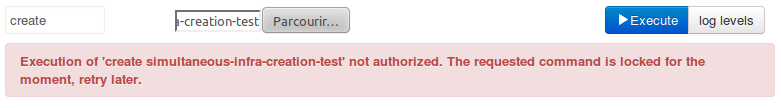
\includegraphics[width=\textwidth]{cmdLocked.png}
  \caption{La commande 'create simultaneous-infra-creation-test' est déjà en
    cours d'exécution.}
\end{figure}

Certaines commandes n'ont pas de verrou car elles n'ont pas d'effet de bord.
Par exemple les commandes status, status-services et show n'ont pas besoin
de verrou car elles ne font que récupérer des informations concernant une infra.

\underline{\textit{Bilan}} : Le verrouillage d'une commande à risque n'est
assuré que si toutes les opérations se font via l'interface web. C'est la webapp
côté serveur qui fait le contrôle. L'outil d'infra en ligne de commande, lui ne
verrouille aucune commande.

\section{Fonctionnalités de la webapp}

\subsection{Complétion automatique des infras}

L'application web fournit une complétion automatique des noms d'infrastructures
pour les champs qui requièrent une infra.

\begin{figure}[H]
  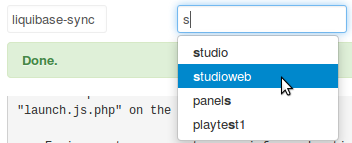
\includegraphics[scale=1]{auto-completion.png}
  \caption{Complétion automatique des noms d'infrastructures disponibles}
\end{figure}

La liste déroulante assiste l'utilisateur lorsqu'il doit indiquer
l'infrastructure sur laquelle s'appliquera sa commande.
Cette fonctionnalité améliore l'expérience utilisateur, l'utilisateur gagne du
temps et évite les erreurs de frappe.

C'est le plugin JavaScript Typeahead de Twitter Bootstrap qui est utilisé pour
avoir ce design sympathique. L'internaute tape quelques lettres de l'item qu'il
recherche et le plugin affiche les items qui contiennent cette séquence de
lettres en facteur.

Une fois le plugin inclus dans le projet, il faut renseigner l'attribut
\textit{data-source} de la balise input avec les différents choix possibles de
la liste.

\lstset{language=XML}
\begin{lstlisting}[caption=utilisation de bootstrap-typeahead]
  <input type="text" data-provide="typeahead" data-items="4" data-source='[]'>
\end{lstlisting}

Comme présenté dans le code html ci-dessus, la liste est vide au début.
Elle contiendra la liste des infras disponibles qui sera générée côté serveur.

Lorsque l'utilisateur se connecte à l'application, la page web lui est envoyée
instantanément. Il peut exécuter la commande qu'il souhaite mais ne
dispose pas encore de la complétion automatique des infrastructures.

Une WebSocket est utilisée pour remplir dynamiquement cette liste.
En asynchrone, la commande \textit{list} est exécutée côté serveur.
Cette commande récupère la liste de toutes les infrastructures disponibles en
requêtant Chef qui dispose de cette information. La commande \textit{list} met
environ 5 secondes à s'exécuter sur l'instance EC2 qui héberge l'application
web.
Une fois la commande \textit{list} terminée, le serveur envoie cette liste des
infrastructures au client via la WebSocket.
Une fonction JavaScript renseigne alors l'attribut data-source avec
la liste des infrastructures reçue.

Le client ne ressent aucune latence de l'application car les briques essentielles
de l'interface web pour exécuter une commande sont instantanément disponibles.
Les fonctionnalités complémentaires comme l'auto-complétion viennent se greffer
dynamiquement à l'interface et n'altèrent pas la navigation de l'utilisateur.

\underline{\textit{Bilan}} : Cette autocomplétion tire pleinement parti du
modèle asynchrone offert par les \textit{WebSocket}. Cette fonctionnalité met
bien en évidence l'intérêt des \textit{WebSocket} pour créer des pages web qui
se mettent à jour dynamiquement en recevant des informations calculées en
asynchrone. Les pages web peuvent devenir de vraies applications temps réel.

\subsection{Défilement automatique des logs de la commande en cours d'exécution}

\begin{figure}[H]
  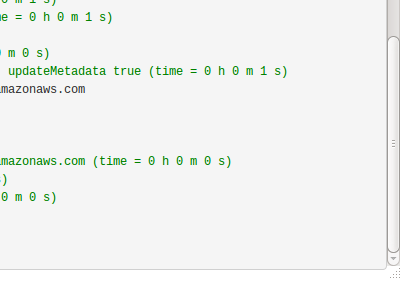
\includegraphics[width=0.50\textwidth]{defilement-automatique-1.png}
  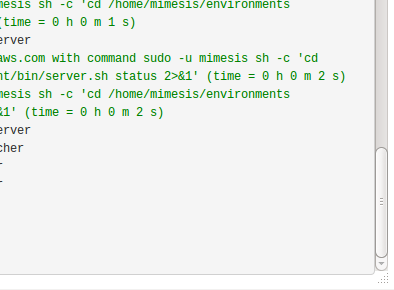
\includegraphics[width=0.50\textwidth]{defilement-automatique-2.png}
  \caption{Défilement automatique des logs - exécution de la commande
    status-services panel\\L'image de droite est prise 4 secondes après celle de gauche}
\end{figure}

Lorsqu'une nouvelle ligne est ajoutée à la suite de l'output du résultat de la
commande, la barre de défilement se met automatiquement en bas.

Si l'utilisateur déplace la barre de défilement, le défilement automatique se
désactive.
Si l'utilisateur replace manuellement la barre de défilement tout en bas,
le défilement automatique est de nouveau actif.

\underline{\textit{Bilan}} : Aucun plugin n'est utilisé ici. Quelques lignes de
JavaScript suffisent pour créer ce système de défilement automatique.

%% \subsection{couleurs des logs}
\subsection{Contrôler les niveaux de log}

Avant d'exécuter une commande, les niveaux de logs peuvent être activés ou
désactivés. Les informations affichées au cours de l'exécution de la commande
sont alors filtrées pour n'afficher que celles correspondant aux niveaux de logs.
Il y a cinq niveaux de logs utilisés dans l'application : 
Trace, Debug, Info, Warn et Error.
Par défaut, tous les niveaux de logs sont activés.

\begin{figure}[H]
  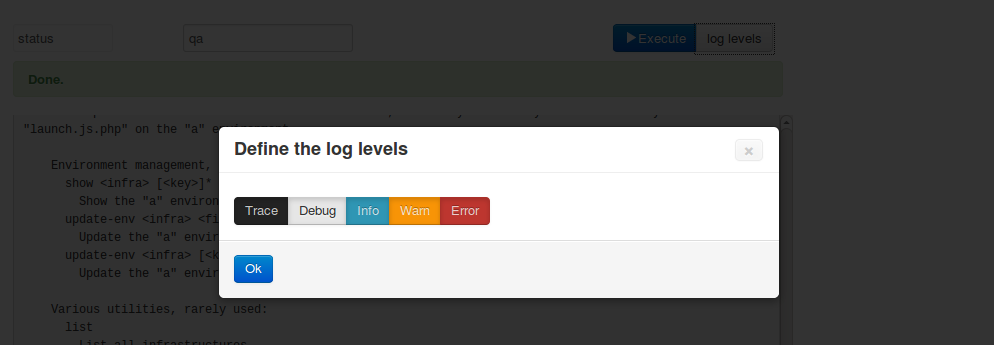
\includegraphics[width=\textwidth]{log-levels.png}
  \caption{Tous les niveaux de logs sont activés}
\end{figure}

\bigskip

La commande \textit{status} fait un appel au logger.debug durant son exécution.
Un utilisateur laissera le niveau Info actif et désactivera Debug
si il souhaite uniquement recevoir le résultat du \textit{status} et ne veut pas
être encombré des tous les logs de Debug.
Du coup, lors de l'exécution de la commande \textit{status qaz}, la ligne
\verb?EXEC: Perform get on data/infrastructures/qaz? ne sera pas affichée car le
niveau Debug a été désactivé par l'utilisateur.

\underline{\textit{Bilan}} : Ce filtrage des niveaux de log est apprécié des
utilisateurs. Il était souvent reproché que la sortie console d'une commande
était beaucoup trop verbeuse. À présent, l'internaute peut régler le niveau de
log à sa convenance.

\subsection{La commande download-chef-log}
La création et la mise à jour d'une infra sont des tâches délicates qui peuvent
souvent échouer.
La cause de cet échec peut varier.
Ça peut venir par exemple de la création de la base de donnée RDS qui ne s'est
pas correctement terminée comme ça peut aussi venir de la limite du nombre de
groupes de sécurité fixée par Amazon qui est atteinte.

Mais la cause la plus fréquente est l'échec de l'exécution du chef-client.
À chaque fois que ce programme plante, un administrateur système doit récupérer le
fichier de logs Chef pour connaître la cause. Il recherche alors sur amazon
l'url de l'instance EC2 qui héberge l'infrastructure car c'est cette instance
qui exécute chef-client et qui possède les logs Chef. Une fois cette url
trouvée, il peut se connecter à l'instance via ssh et récupérer le fichier de
log.

Pour éviter cette tâche fastidieuse aux administrateurs systèmes, la commande
\textit{download-chef-log} a fait son apparition dans l'application web.

Depuis l'interface web, il suffit de renseigner deux champs pour récupérer le
fichier de log. Un premier champ doit contenir le nom de l'infrastructure et un
deuxième doit contenir le nom du nœud sur lequel la commande a échoué.

Contrairement à l'url de l'instance qui n'était pas connu par l'administrateur
système et qu'il devait rechercher sur Amazon, il connaît déjà le nom d'infra et
le nom du nœud.

De plus, pour faciliter son utilisation, les deux champs de cette nouvelle
commande \textit{download-chef-log} possèdent la complétion automatique.

\begin{figure}[H]
  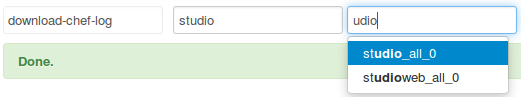
\includegraphics[width=\textwidth]{completion-download-chef-log.png}
  \caption{Complétion automatique disponible aussi pour la liste des nœuds}
\end{figure}

À partir du nom de l'infra et du nœud, le serveur web requête Chef pour
connaître l'url de l'instance EC2 correspondante. En utilisant la commande
\textit{scp}, le serveur copie le fichier de logs Chef distant dans un
dossier local publique.
L'application génère ensuite une URL qui pointe sur le fichier local téléchargé
et envoie cette URL au client.
L'URL est alors affichée sur la page web de l'utilisateur. Il lui suffit de
cliquer dessus pour télécharger le fichier de log qu'il recherchait.


\begin{figure}[H]
  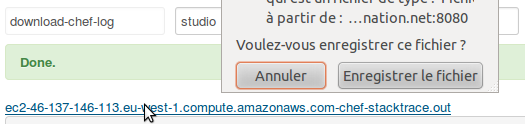
\includegraphics[width=\textwidth]{download-chef-log.png}
  \caption{Lien de téléchargement du fichier de log généré par la commande \textit{download-chef-log}}
\end{figure}

\underline{\textit{Bilan}} : Cette commande est principalement utilisée par les
administrateurs système de la société. Cependant, ils ne peuvent pas se servir
de l'outil en ligne de commande pour l'exécuter car elle n'existe que pour
l'application web.

\section{Évolutions de l'outil d'infra}

\subsection{Création d'infrastructure}

\subsubsection{Des logs plus complets}

Lors de la création d'infra, l'outil appelle le programme \textit{chef-client}
sur chaque instance EC2 de l'infra. 

\underline{\textit{L'objectif}} : Récupérer les logs de la commande chef-client
en cours d'exécution sur l'instance EC2 distante pour pouvoir les afficher à
l'utilisateur.

Le programme \textit{chef-client} initialise toutes les données Chef.
C'est aussi l'étape qui prend le plus de temps à s'exécuter lors d'une création
d'infrastructure.

Une session ssh est ouverte avec la lib Java jsch sur l'instance EC2 qui va
exécuter le chef-client. On ouvre un channel de type \textit{exec} sur lequel on
définit notre logger et la commande à exécuter (i.e. \textit{chef-client}).

\underline{\textit{Bilan}} : Un point négatif est que les logs du
\textit{chef-client} sont assez volumineux. Le client de l'outil d'infra 
peut donc être submergé par toutes ces informations. À trop voir de détails, on
finit par les ignorer. Mais tout de même, lorsqu'une erreur se produit,
l'utilisateur dispose maintenant de toutes les informations d'exécution puisque
tous les logs de n'importe quel programme externe appelé par l'outil d'infra
sont affichés.

%% - afficher les logs du chef-client dans la sortie web lors d'une création
%% d'infra.

\subsubsection{Un nouveau groupe de sécurité de RDS pour chaque nouvelle infra}

L'outil d'infra utilisait le groupe de sécurité RDS par défaut pour les bases de
données associées à une instance. Un nombre limité d'instances EC2 peut être
associé à un groupe de sécurité RDS et cette limite éteinte.

\underline{\textit{L'objectif}} : Créer un nouveau groupe de sécurité RDS pour chaque
\textit{create} d'une nouvelle infra. 

La priorité est haute car la création d'une nouvelle infrastructure ne
fonctionne plus. Le patch est rapidement créé et une nouvelle version de l'outil
d'infra est publiée pour que tout le monde puisse de nouveau créer une
infrastructure avec l'outil.

\underline{\textit{Bilan}} : L'ajout du code pour ce patch dans le temps imparti
montre que je maîtrise à présent le code de l'outil d'infra.

%% - J'ai écris le code qui créé un nouveau db security group rds à chaque fois
%% qu'une nouvelle infra est créée.
%% Ça permettra d'éviter la limite qu'on atteint rapidement lorsqu'on utilise le
%% security group 'default'.


\subsubsection{Des vérifications supplémentaires au début de l'exécution}

\underline{\textit{L'objectif}} : Rajouter des vérifications au début de
l'exécution de la commande \textit{create} pour éviter qu'elle n'échoue plus
tard dans l'exécution.

\begin{itemize}
\item[\textbullet] Les instances de type \textit{t1.micro} n'ont pas assez de
  mémoire pour héberger une infra MambaNation.
  À présent, l'outil d'infra peut détecter et interdire la création d'une
  infrastructure sur ce type d'instance Amazon dès le début de l'exécution de la
  commande \textit{create}.
\item[\textbullet] Une autre vérification empêche la création d'infrastructure
  dont le nom contient une majuscule car les noms avec majuscules ne sont pas
  autorisés pour les Bucket S3.
\end{itemize}


\underline{\textit{Bilan}} :  Il ne sert à rien d'exécuter une création d'une
infrastructure s' il est possible de détecter à l'avance qu'elle va échouer.  
Ces vérifications permettent de détecter une erreur plus tôt et d'afficher des
messages d'erreurs court et explicites.

%% - J'ai rajouté un check dans l'outil d'infra pour interdire le create sur une
%%  parce-que la création d'infra sur une t1.micro ne fonctionne pas, pas
%% assez de mémoire disponible sur les micros probablement.
%% J'ai rajouté un autre check qui vérifie que le nom de l'infra ne contient pas de
%% majuscule.


%% - J'ai fait en sorte de pouvoir créer des infras même sans service mongodb.


\subsection{Optimisations en temps d'exécution}

La commande \textit{registerDns} enregistre un nouveau nom DNS sur AWS Route53
pour chaque nœud de l'infrastructure précisée en entrée de la
commande. \textit{registerDns} met ensuite à jour Chef pour indiquer les
nouveaux DNS assignés.

\subsubsection{Exécution parallèle}

Les enregistrements de ces noms de domaine sont indépendants les uns des autres.
Cette commande a donc été modifié pour que \underline{chaque enregistrement DNS
  s'exécute en parallèle des autres}.

\subsubsection{La manière d'utiliser cette méthode ne change pas}

La méthode registerDns correspondant à la commande du même nom possède un point
de jointure à la fin de son code. Bien que tous les enregistrements soient
effectués en parallèle, la méthode s'assure que tous les enregistrements DNS
sont bien terminés au niveau du point de jointure. 
Ainsi l'utilisateur de la méthode registerDns peut chaîner un appel à une autre
méthode avec la certitude que cette deuxième méthode ne sera appelée uniquement
si tous les enregistrements DNS se sont bien exécutés.

La manière d'utiliser cette méthode ne change pas pour l'utilisateur et le
nouveau code source de la méthode reste compatible avec le reste du code
existant de l'outil.

\subsubsection{Implémentation}

Toutes les classes de l'outil d'infra utilisent la bibliothèque des
\textit{Promises} de MimesisRepublic.
Les \textit{Promises} sont une bonne solution pour exécuter plusieurs opérations
en parallèle d'une manière efficace et non bloquante.

La type de retour de la méthode registerDns est
\textit{Promise[StartedInfrastructure]}.

L'instance de StartedInfrastructure contenue dans la Promise retournée
représente la nouvelle infrastructure dont les DNS ont bien été enregistrés.
Cette Promise contient une StartedInfrastructure qui n'existe pas encore mais
qui pourra être récupérée plus tard.
Voici le code source de la méthode registerDns avec des commentaires rajoutés en
français pour détailler ce qu'elle fait.
\lstset{language=Scala}
\begin{lstlisting}
  class StartedInfrastructure {
    ...

    def registerDns() : Promise[StartedInfrastructure] = 
    logger.logPromOp("Register DNS for infrastructure percentageSigns".format(infraName)) {

      // la méthode join est notre point de jointure.
      def registerAllDns = Promise.join(startedNodes.map { node => node.registerDns(infraName, topDomain) }.toList)

      // méthode qui met a jour l'attribut db_servers_list dans Chef.
      def updateDbServerList() : Unit =
      getNodeWithRole("mongodb_server").headOption.map { 
        node =>
        val newBrmStructure = dbServersList("brm").updated("host", node.privateIp)
        .updated("server_id", node.nodeName)

        val newDbServersList = dbServersList.updated("brm", newBrmStructure)
        structure = structure.updated("db_servers_list", newDbServersList)
        val json = Json.build(structure)
        chef.saveDataBagItem(rootDataBagPath, infraName, json)
      }

      // chaînage des différentes tâches avec la méthode map de la classe Promise :
      // tous les enregistrements DNS sont effectués (registerAllDns) puis les
      // données sont mises à jour dans Chef (updateDbServerList) puis l'instance 
      // de StartedInfrastructure est retournée (this).
      registerAllDns.map { xs => updateDbServerList(); xs }.map(xs => this)
    }
  }
\end{lstlisting}

\underline{\textit{Bilan}} : La méthode registerDns est exécutée par plusieurs commandes
dont \textit{create}, \textit{start}, \textit{restart-services} et
\textit{registerDns}. L'optimisation de cette méthode permet par exemple de
gagner environ 10 secondes lors de la création d'une infra avec quatre nœuds.

\subsection{Documentation dans le wiki}

Certaines commandes de l'outil d'infra échouent plus souvent que
d'autres car elles effectuent des opérations délicates tels que le démarrage
d'instance EC2 et l'écriture en base de données. Les commandes de création et de
destruction d'infrastructure, \textit{create} et \textit{destroy}, en font
partie.

Lorsqu'une commande échoue, les logs affichés à l'utilisateur de l'outil d'infra
(en ligne de commande ou web) décrivent son déroulement pas à pas. Mais parfois
les logs ne suffisent pas et sans une bonne connaissance de l'ensemble des
étapes exécutées par ces lourdes commandes, il est très dur de découvrir la
cause de l'échec.

\underline{\textit{La demande :}} documenter le déroulement des commandes \textit{create},
\textit{destroy}, \textit{start} et \textit{stop}.

Toutes les étapes de ces quatre commandes ont donc été documentées dans le wiki
de Mimesis. Cette page de documentation permet de savoir si l'enregistrement des
DNS s'effectue avant ou après l'initialisation de la base de données RDS ou
encore de savoir à quel moment la liste des services est ajoutée dans Chef par
exemple.
L'utilisateur a ainsi une vision plus claire du déroulement de l'exécution de
l'outil d'infra.
Un administrateur système peut se servir de cette documentation pour repérer
l'opération qui a échoué et la réparer manuellement.

\underline{\textit{Bilan}} : La documentation est nécessaire pour garder une certaine
maîtrise sur le travail effectué. Une fois écrite, la documentation offre aussi
une certaine autonomie aux employés. \\
Travaillant sur l'outil d'infrastructure tous les jours, j'ai moi même découvert
des subtilités dans le déroulement de la commande \textit{create} que je ne
connaissais pas. Cette page de documentation permet à tout le monde d'y voir
un peu plus clair sur l'exécution de l'outil d'infra et sert de premier support
lorsqu'une commande échoue.

\section{Plugin SBT}

Afin de faciliter le déploiement d'un service, Mimesis Republic a mis en place
un modèle de déploiement uniforme sur l'ensemble des infrastructures pour tous
les composants applicatifs.

Tout projet packagé dans une archive zip doit respecter une arborescence bien
définie et l'application web Play! n'y échappe pas.

Un fois dézippé, le projet doit avoir la structure suivante :
\begin{itemize}
\item[\textbullet] conf    (contient les fichiers de configurations)
\item[\textbullet] app     (contient les fichiers binaires)
\item[\textbullet] scripts (contient les scripts)
\end{itemize}

Le dossier \textit{scripts} doit contenir un fichier service.sh .
Ce script permet de démarrer, arrêter, redémarrer ou récupérer l'état de
l'application en question.
Son utilisation est simple :
\begin{lstlisting}
  Usage: service.sh { start | stop | restart | status }  
\end{lstlisting}

Les équipes de la société ont créé plusieurs plugins SBT pour automatiser le
packaging de tout type d'application utilisée.
Ainsi, dans n'importe quel sous-projet de la société (projet PHP, Rails ou
autres), pour créer un zip de l'application courante qui respecte la
structure imposée, il suffit de :
\begin{itemize}
\item ouvrir un terminal
\item invoquer l'interpréteur de commandes \textit{sbt}
\item taper la commande \verb?playad-bundle-generate(for standalone)? \\
\end{itemize}

Jusqu'à présent, Mimesis Republic n'avait pas de projet Play! en développement.
Il n'y avait donc pas de plugin SBT existant pour Play!. 
Le plugin SBT PlayadPlayPlugin a donc été créé pour offrir ce packaging 
automatique.
Désormais, la commande \verb?playad-bundle-generate(for standalone)? fonctionne
aussi pour l'application web \textit{infra-admin-web}.
Une fois l'archive dézippée, le dossier \textit{infra-admin-web} contient bien
les dossiers conf, app et scripts avec le script service.sh pour piloter le
serveur web de l'application.

\underline{\textit{Bilan}} : Le modèle de déploiement uniforme est une très
bonne idée. Le démarrage ou l'arrêt d'une application quelconque peut alors être
 automatisé par un outil externe. 
À présent, pour tout projet Play! à venir, il suffira d'utiliser le plugin
\textit{PlayadPlayPlugin} pour pouvoir accéder à la commande qui package
l'application.
Ça n'a pas été simple de coder ce plugin \textit{PlayadPlayPlugin} car SBT nous
force à configurer des composants immuables au travers de Monads. C'est un style
de programmation très proche des langages fonctionnels et très éloigné des
langages impératifs auxquels j'étais habitué. Malgré son nom (Simple Build
Tool), SBT n'est pas n'est pas si simple après tout.


